%!TEX root = Main.tex
\section{Tests}
This section contains descriptions of the tests done as part of the mini project.

\subsection{Compression}
The algorithms were first designed and implemented in C and tested on a PC since debugging is easier on the PC.
Afterwards the code was implemented in nesC and tested on the TelosB.
The purpose of this integration test was to validate that the algorithms worked correctly on the TelosB before we ran the full system test.
This was done by letting the TelosB compress, and decompress the image in flash on boot.
After transferring an image to the flash, and then rebooting, the compressed image can be read out of the flash. By using MATLAB it was then possible to verify that the algorithm preformed as expected.

\subsection{Full System Test}
\label{subs:FST}

The purpose of this test was to validate the compression -> sending -> decompression procedure before measurements are done.
The image was sent between the TelosB motes once for each compression algorithm.
The image was then transferred to a computer and compared with a correctly compressed and decompressed image in MATLAB.

\subsection{Energy Measurements}
To measure the energy used by the TelosBs, the test setup in figure \ref{fig:EnergyTestSetup} was used. 

\begin{figure}[H]
	\centering
	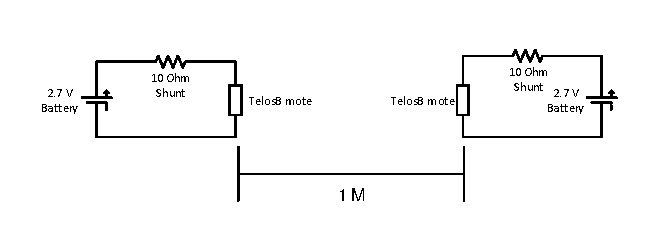
\includegraphics[scale=1] {TestSetup}
	\caption{Energy Test Setup}
	\label{fig:EnergyTestSetup}
\end{figure}

Using a oscilloscope the voltage over the 10 ohm shunt is measured on both sender and receiver.The battery voltage is also measured for both motes. For each compression algorithm 3 measurements were done on both sender and receiver. The measured data can be seen in the table \ref{tab:MeasurementResults}. If a packet error was observed during the measurements,  this measurement discarded. This is done to make the measurements more comparable.



\section{Results}
This section contains the results of the tests done during the mini project.

Before the energy measurements are made, the functionality was validated. Using the test setup in section \ref{subs:FST}, an image was written to the flash, and then compressed and sent. 

\begin{figure}[H]
	\centering
	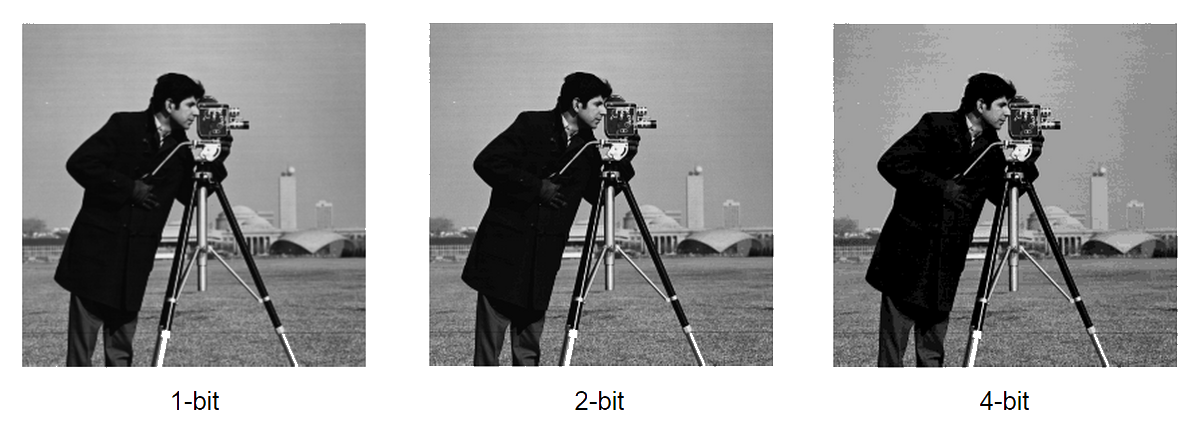
\includegraphics[width=0.8\textwidth] {cameramanresult}
	\caption{Compression Results}
	\label{fig:cameramanresult}
\end{figure}

The compressed images can be seen on figure \ref{fig:cameramanresult}. To ensure that the compression-send-decompress procedure was successful it is compared with the same image compressed and decompressed in Matlab. By comparing this two images it is shown that the functionality is as expected. 


Looking at the voltage over the shunt, we can see how the system uses power, for the test setup a typical power over time is illustrated in figure \ref{fig:ImageTransfere}.

\begin{figure}[H]
	\centering
	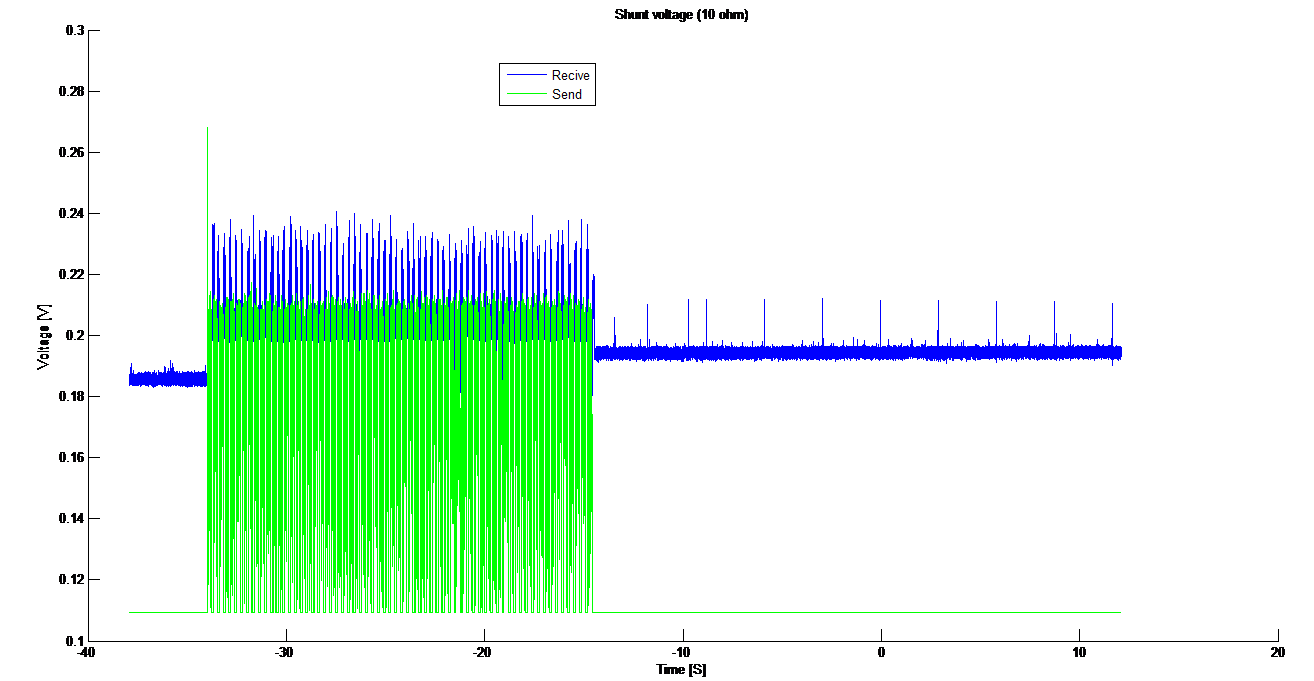
\includegraphics[width=1\textwidth ]{ImageTransfere}
	\caption{ Shut voltage during image transfer. }
	\label{fig:ImageTransfere}
\end{figure}

For each compression algorithm 3 measurements was done on both sender and receiver. 
The measurements can be seen in the table \ref{tab:MeasurementResults}.


\begin{table}[h]
	\begin{tabular}{cllllll}

	\cline{2-5} 
	\multicolumn{1}{l}{} 	& \multicolumn{2}{l}{Energy {[$J$]}} & \multicolumn{2}{l}{Mean Power [$W$]} &	&	\\ \hline
	\rowcolor{gr}
	\multicolumn{1}{l}{Bit Removed}	& Sender	& Receiver	& Sender	& Receiver	& \multicolumn{1}{l}{Transfer Time [$S$]} & \multicolumn{1}{l}{Better Power Than None} \\ \hline
	% \rowcolor{gr}
	\multicolumn{1}{c}{\multirow{3}{*}{None}} & 0,988	& 1,131	& 0,043	& 0,049	& \multicolumn{1}{l}{23,0}	& \multicolumn{1}{l}{0\%}	\\  
	\multicolumn{1}{c}{}	& 0,990	& 1,133	& 0,043	& 0,049	& \multicolumn{1}{l}{23,0}	& \multicolumn{1}{l}{0\%}	\\ 
	% \rowcolor{gr} 
	\multicolumn{1}{c}{}	& 0,985	& 1,130	& 0,043	& 0,049	& \multicolumn{1}{l}{23,0}	& \multicolumn{1}{l}{0\%}	\\ \hline
	% \rowcolor{gr} 
	\multicolumn{1}{c}{\multirow{3}{*}{One}}  & 0,879	& 1,047	& 0,042	& 0,049	& \multicolumn{1}{l}{21,2}	& \multicolumn{1}{l}{8\%}	\\ %\cline{2-7} 
	\multicolumn{1}{c}{}	& 0,879	& 1,047	& 0,042	& 0,049	& \multicolumn{1}{l}{21,2}	& \multicolumn{1}{l}{8\%}	\\ %\cline{2-7} 
	% \rowcolor{gr} 
	\multicolumn{1}{c}{}	& 0,879	& 1,046	& 0,042	& 0,049	& \multicolumn{1}{l}{21,2}	& \multicolumn{1}{l}{8\%}	\\ \hline
	% \rowcolor{gr} 
	\multicolumn{1}{c}{\multirow{3}{*}{Two}}  & 0,799	& 0,964	& 0,041	& 0,050	& \multicolumn{1}{l}{19,5}	& \multicolumn{1}{l}{15\%}	\\ %\cline{2-7} 
	\multicolumn{1}{c}{}	& 0,800	& 0,966	& 0,041	& 0,050	& \multicolumn{1}{l}{19,5}	& \multicolumn{1}{l}{15\%}	\\ %\cline{2-7} 
	% \rowcolor{gr}
	\multicolumn{1}{c}{}	& 0,800	& 0,965	& 0,041	& 0,050	& \multicolumn{1}{l}{19,5}	& \multicolumn{1}{l}{15\%}	\\ \hline
	% \rowcolor{gr}
	\multicolumn{1}{c}{\multirow{3}{*}{Four}} & 0,591	& 0,744	& 0,040	& 0,050	& \multicolumn{1}{l}{14,9}	& \multicolumn{1}{l}{35\%}	\\ %\cline{2-7} 
	\multicolumn{1}{c}{}	& 0,591 & 0,743	& 0,040	& 0,050	& \multicolumn{1}{l}{14,9}	& \multicolumn{1}{l}{35\%}	\\ %\cline{2-7} 
	% \rowcolor{gr}
	\multicolumn{1}{c}{}	& 0,600 & 0,742	& 0,041	& 0,050	& \multicolumn{1}{l}{14,9}	& \multicolumn{1}{l}{35\%}	\\ \hline
	\end{tabular}

	\caption{Measurement Results }
	\label{tab:MeasurementResults}
\end{table}
